\chapter{Vectorization}\label{chp:vectorization}
Vectorization, raster-to-vector conversion or image tracing is the conversion of raster graphics to vector graphics. To understand the reason for converting from raster to vector we need to look at some of the properties of both storage techniques.

Raster data is structured as an array of grid cells, also referred to as pixels. Each cell in a raster can be addressed by its position in the array, by row and column number. Since each pixel has it's own value, a raster can represent a range of spatial objects. A point can be represented by a single pixel, an arc represented by a sequence of pixels and an area as a collection of continuous pixels. Vector data is structured as a finite straight line segment defined by its endpoints. The location, or coordinates, of the endpoints, are given with respect to a coordinatization of the plane. The vector representation is not discretized in a grid space the same way as a raster but does follow an implicit grid structure as a result of the nature of computer arithmetic. Like the raster, the vector structure can represent multiple spatial structures. A point is given by its coordinates, an arc represented as a sequence of line segments, each consisting of start and end coordinates and an area represented by its boundary consisting of a collection of vectors.

\begin{figure}[H]
	\centering
	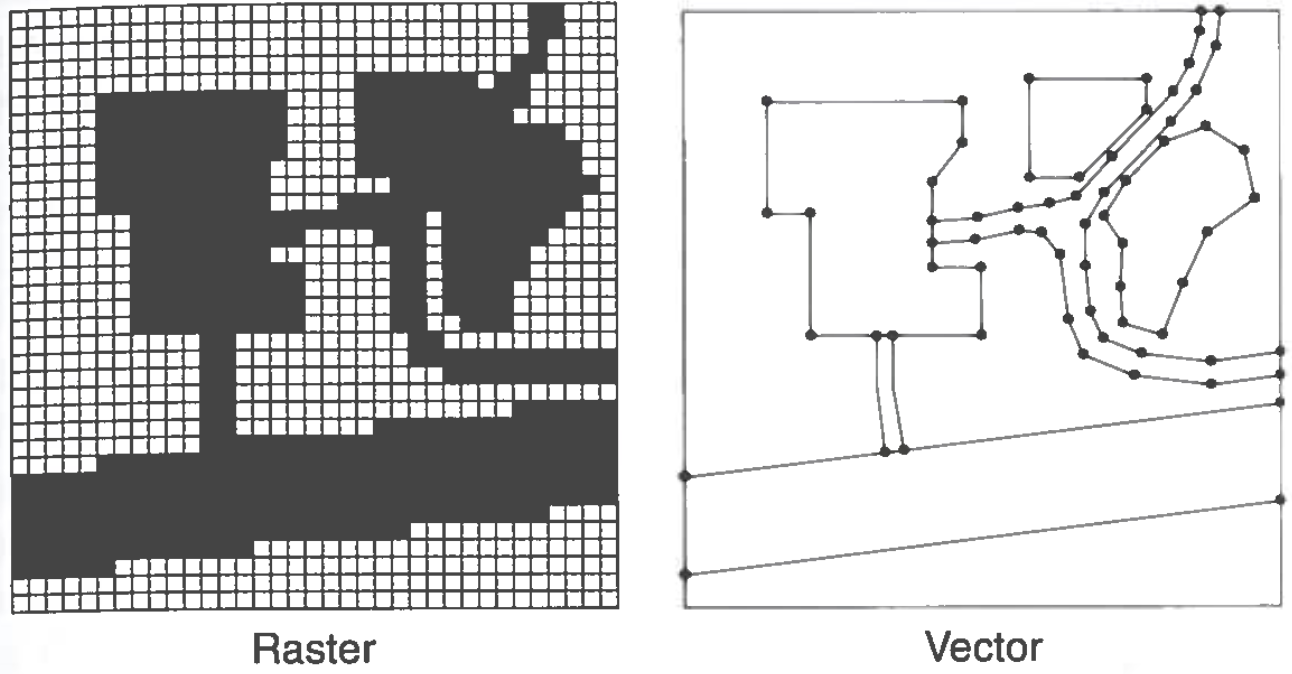
\includegraphics[width=0.8\linewidth]{fig/rastervector.png}
	\captionsource{Raster and vector data}{\citet{Worboys2003}}
	\label{fig:rastervsvector}
\end{figure}

There are multiple reasons for storing data in vector format: The geographic accuracy is higher since it is not dependent on grid size, it allows for efficient encoding of topology, an important aspect when doing analysis that utilizes topologic relations, such as proximity and network analysis and it allows for storage of attributes in the data, giving us another dimension of information and the storage size is smaller.

There are multiple different techniques for vectorization. We will now look at some of the well-known ones.

\section{Hough Transform}
The Hough Transform can isolate features of particular shape within images. The user must describe the desired feature in a parametric form, therefore the most common application of Hough Transform is to detect regular curves such as lines and circles. The technique is known to be tolerant of image noise and gaps in the feature boundary.

Hough Transform works by transforming each of the pixels into a straight line in a parameter space. The parameter space is described by the parametric form of features we are looking for. In the simplest case of a Hugh Transform, we want to detect straight lines. For this the normal form $r = x cos(\theta) + y sin(\phi)$ is used to represent the lines. When iterating the pixels in the image the algorithm looks if there is enough evidence that there is a straight line at that pixel, if there is, it calculates the parameters $\theta$ and $\phi$ at that point and adds it to an array. The array accumulates all the points that belong to each specific $\theta$ and $\phi$, thus the more points that are on the same parameters the more likely they belong to a line. The algorithm visits each pixel one time and is therefore linear with the number of pixels in the image.

\section{Thinning}
Thinning is a morphologic operation that is used to remove foreground pixels from an image, resulting in a simplified image with the same topological relations as the input image. It works by successively removing pixels from the boundary until there is not possible to remove more. The skeleton that is left contains the centerlines of the objects. This technique is mostly used on binary images. The iterative nature of the algorithm makes it computationally expensive.

\section{Contour}
This method aim at lowering the computational cost compared to thinning. The main idea is to find edges before calculating the middle point that is between two opposite parallel edges. A chain of middle points represents the medial axis. It has to use an edge detection algorithm before extracting the middle points between the edges. A problem with the contour based methods is how they deal with junctions. It is likely to miss junctions that are crossing at a small angle and it has difficulties with cross intersections where four lines meet \cite{Wenyin1999}. It is thus not suited for vectorization of curves and crossing lines.

\section{Run-graph}
Run-graph is a semi-vector representation of the raster image \cite{Monagan1993}. It examines the raster in either row or column direction in what is defined as horizontal and vertical \emph{runs}. A horizontal run is a maximal horizontal sequence of black pixels. A vertical run is a maximal vertical sequence of black pixels. After running, the run-graph is composed of edge areas that represent line segments and node areas and touching points that correspond to endpoints and junctions. The line extraction from the graph attempts to minimize the area of the node and maximize the length of the connected edges. Run-graph based methods are vulnerable to image noise and can cause unsatisfactory results at junction areas \cite{Karabork2008}.

\section{Mesh pattern}
Mesh pattern was introduced by \citet{Lin1985}. The idea is to divide the image into a mesh and check the distribution of black pixels at the border of each mesh unit. Using the patterns along the border, a control map is created. Lines are then extracted from the control maps by comparing them to characteristic patterns in a pattern database. Unknown patterns are labeled with question marks. These areas are analyzed pixel by pixel to determine where the line goes. In \autoref{fig:meshpattern} we can see the process of generating a mesh, extracting the control maps and filling the lines based on the analysis of control maps. 

\begin{figure}[H]
	\centering
	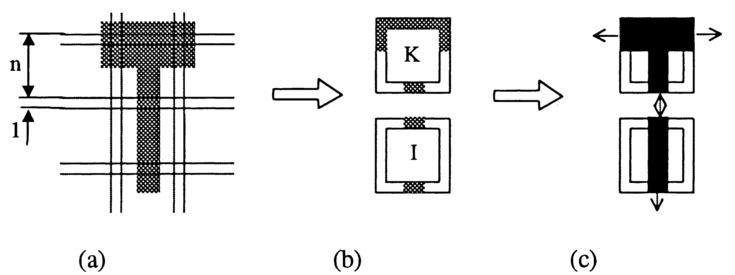
\includegraphics[width=0.8\linewidth]{fig/meshpattern.png}
	\captionsource{Mesh pattern line extraction. (a) image and mesh, (b) mesh pattern labels and control map, (c) lines extracted by analyzing the control map.}{\citet{Wenyin1999}}
	\label{fig:meshpattern}
\end{figure}

\section{Sparse-pixel}
The first of these algorithms was the Orthogonal Zig-Zag (OZZ) introduced by \citet{Dori1997}. The basic idea of the algorithm is to track a single pixel wide "beam of light" which turns orthogonally each time it hits an edge, the same way light travels in a fiber-optic cable. In the algorithm, the beam changes direction if it encounters white pixels or the length of the beam exceeds a predefined threshold. If the threshold is hit, two new beams are emitted orthogonally from the point. This can be seen in \autoref{fig:zigzag}. The midpoint of the runs are also recorded, used to reconstruct the line, corner correction and merger of crossing lines. \citet{Wenyin1996} improved the OZZ method with Sparse Pixel Vectorization (SPV). There were three main improvements: The procedure begins with a reliable medial axis point found by a separate procedure for each black area, a general following procedure is used for all cases of OZZ, i.e. Vertical, horizontal and diagonal following and a junction recovery procedure is applied whenever a junction is encountered during following.

\begin{figure}[H]
	\centering
	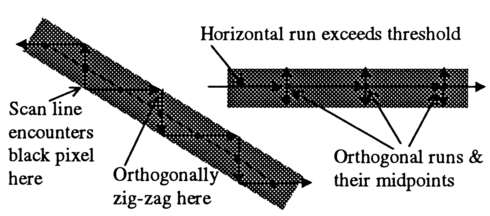
\includegraphics[width=0.8\linewidth]{fig/zigzag.png}
	\captionsource{Orthagonal Zig-Zag}{\citet{Wenyin1999}}
	\label{fig:zigzag}
\end{figure}